\documentclass[conference]{IEEEtran}

\makeatletter
\def\ps@IEEEtitlepagestyle{%
  \def\@oddfoot{\mycopyrightnotice}%
  \def\@evenfoot{}%
}
\def\mycopyrightnotice{%
  {\footnotesize XXX-X-XXXX-XXXX-X/XX/\$XX.00~\copyright~20XX IEEE\hfill}%
  \gdef\mycopyrightnotice{}%
}
\makeatother

\IEEEoverridecommandlockouts

\usepackage{cite}
\usepackage{amsmath,amssymb,amsfonts}
\usepackage{algorithmic}
\usepackage{graphicx}
\usepackage{textcomp}
\usepackage{xcolor}
\usepackage{eso-pic}
\usepackage{booktabs}
\usepackage{threeparttable}
\usepackage{multirow}
\usepackage{url}
\usepackage{tikz}
\usepackage{hyperref}
\usetikzlibrary{shapes.geometric, arrows.meta, positioning, calc}

\def\BibTeX{{\rm B\kern-.05em{\sc i\kern-.025em b}\kern-.08em
    T\kern-.1667em\lower.7ex\hbox{E}\kern-.125emX}}

\newcommand\AtPageUpperMyright[1]{\AtPageUpperLeft{%
 \put(\LenToUnit{0.17\paperwidth},\LenToUnit{-2cm}){%
     \parbox{0.9\textwidth}{\raggedleft\fontsize{8}{11}\selectfont #1}}%
 }}%
\newcommand{\conf}[1]{%
\AddToShipoutPictureBG*{%
\AtPageUpperMyright{#1}%
}%
}

\begin{document}

\title{\vspace{1cm} Simulating Brazilian Public Opinion with Large Language Models: Distributional Evaluation and Prompt Engineering}

\author{
\IEEEauthorblockN{1\textsuperscript{st} Lucas Nascimento Aguiar}
\IEEEauthorblockA{\textit{Graduate Program in Applied Computing} \\
\textit{Mackenzie Presbyterian University (UPM)}\\
São Paulo, Brazil \\
lucas.naguiar@outlook.com.br}
\and
\IEEEauthorblockN{2\textsuperscript{nd} Matheus dos Santos Moreira}
\IEEEauthorblockA{\textit{Graduate Program in Applied Computing} \\
\textit{Mackenzie Presbyterian University (UPM)}\\
São Paulo, Brazil \\
matheusmoreira2004@live.com}
\and[\hfill\mbox{}\par\mbox{}\hfill]
\IEEEauthorblockN{3\textsuperscript{rd} Rogério De Oliveira}
\IEEEauthorblockA{\textit{Computing and Informatics} \\
\textit{Mackenzie Presbyterian University (UPM)}\\
São Paulo, Brazil \\
rogerio.oliveira@{mackenzie,maua}.br}
}

\maketitle
\conf{\textit{Proc. of International Conference on Artificial Intelligence, Computer, Data Sciences and Applications (ACDSA 2027) \\ 
2-4 February 2027, Rio de Janeiro-Brazil}}

\begin{abstract}
Simulating public opinion using Large Language Models (silicon sampling)
offers a scalable alternative to traditional polling, yet Global South
contexts remain severely understudied. In this paper, we evaluate whether
Brazilian Portuguese-centric models and global baselines can reproduce
empirical public opinion distributions in Brazil. Grounded in official census
microdata (IBGE) and benchmarked against an empirical survey on Brazilian
perceptions of democracy, we evaluate distributional alignment via
Jensen-Shannon Divergence (JSD). Cumulative prompt engineering --- integrating
feature selection, Chain-of-Thought reasoning, and in-context calibration ---
substantially reduced distributional divergence, achieving optimal alignment
($\text{JSD} < 0.15$). Furthermore, Brazilian models demonstrated superior
sociocultural fidelity by better capturing local civic skepticism compared to
global baselines.
\end{abstract}

\begin{IEEEkeywords}
Large language models, silicon sampling, prompt engineering,
synthetic populations, distributional alignment, sociocultural bias.
\end{IEEEkeywords}

\section{Introduction}\label{sec:introduction}
Public opinion polling constitutes a fundamental instrument for understanding
sociopolitical demands, formulating public policies, and analyzing electoral
behavior. However, traditional field survey methods face increasing logistical
and operational challenges, including high financial costs, lengthy data
collection periods, and declining response rates. In this context, the rapid
advancement of Large Language Models (LLMs) enabled the emergence of
computational approaches directed toward human behavior simulation and synthetic
sampling (\textit{silicon sampling})~\cite{argyle_out_2023}. When conditioned on
sociodemographic attributes, such models exhibit the capacity to emulate
population attitudes and preferences at scale and on demand.

Seminal studies demonstrated that LLMs conditioned on sociodemographic profiles
can reproduce public opinion distributions with remarkable fidelity against real
empirical data~\cite{argyle_out_2023,miranda_simulating_2025}. Nevertheless, the
vast majority of existing literature focuses on North American or European
populations and on models predominantly trained in the English language. A
significant research gap remains regarding the applicability and
transferability of these methodologies to the Brazilian sociocultural context,
as well as the comparative efficacy between general-purpose global models and
models trained with an emphasis on Brazilian sociocultural and political reality.

In this paper, we investigate the ability of Brazilian Portuguese-centric
models against widely adopted global baselines to reproduce empirical public
opinion distributions in Brazil. We construct a
synthetic population comprising 2,000 personas derived from official microdata
provided by the Brazilian Institute of Geography and Statistics (IBGE),
covering demographic, economic, health, and social variables. We adopt the
survey on Brazilian perceptions of democracy conducted by the Center for Public
Opinion Research (CESOP --- \textit{Centro de Estudos de Opinião Pública da
Universidade Estadual de Campinas}) and IPEC~\cite{cesop04832} as the empirical
ground truth. We evaluate the distributional
alignment of the simulated responses using the Jensen-Shannon Divergence
(JSD)~\cite{lin_divergence_1991}.

Our primary contributions are threefold: first, we analyze an experimental
progression of four prompt engineering strategies, demonstrating that combining
feature selection, system/user role separation, Chain of Thought (CoT),
and few-shot calibration reduces JSD divergence by 77\% (from $0.525$ to $0.121$)
to achieve optimal distributional convergence; second, we conduct a systematic
architectural benchmark comparing Brazilian Portuguese-centric models
(Sabiá-4 and Sabiazinho-4) with global baselines (GPT-5-mini and LLaMA~3.2~3B),
revealing that models tailored to the Brazilian reality capture civic skepticism
with higher fidelity, whereas global models exhibit marked social desirability
and institutional optimism biases; and third, we demonstrate the utility of
Explainable Artificial Intelligence (XAI) by employing model-generated
justifications to audit persona reasoning consistency and detect cognitive
dissonances during simulation.\footnote{Replication code, prompt templates,
and evaluation pipelines are available at
\url{https://github.com/olucasaguiar/silicon-sampling-brazil}.}

The remainder of this paper is organized as follows: Section~\ref{sec:related_work}
reviews the theoretical foundation and related work; Section~\ref{sec:methodology}
details the experimental methodology, synthetic sampling procedures, and prompt
engineering scenarios; Section~\ref{sec:results} presents the quantitative
findings, bias analysis, and interpretability discussions; finally,
Section~\ref{sec:conclusion} summarizes the conclusions and outlines directions
for future research.


\section{Theoretical Foundation and Related Work}\label{sec:related_work}
The simulation of human attitudes through Large Language Models (LLMs) has
established a new paradigm in computational social science, termed
\textit{silicon sampling}~\cite{argyle_out_2023,filippas_large_2024}. Autoregressive
models encode latent socio-behavioral priors capable of reproducing collective
demographic viewpoints~\cite{argyle_out_2023,grossmann_ai_2023}, outperforming
classical classifiers in aggregate opinion alignment~\cite{miranda_simulating_2025}.
However, commercial foundation models disproportionately reflect educated, affluent,
and progressive Western strata~\cite{santurkar_whose_2023,bisbee_synthetic_2024},
underrepresenting Global South viewpoints~\cite{durmus_towards_2023} and
exhibiting persistent Anglo-American cultural skews in social and political value
judgments~\cite{hartmann_political_2023,masoud_cultural_2023,johnson_ghost_2022}.
Consequently, faithful simulation in non-WEIRD contexts requires culturally
grounded personas, structured prompt engineering, and empirical calibration.

Bridging demographic profiles with faithful decision-making demands disciplined
prompt design. While LLM execution can be conceptualized as persona role-play
over a generative distribution~\cite{shanahan_role_2023}, unconstrained persona
assignment risks caricaturization and stereotyping~\cite{deshpande_toxicity_2023,salewski_-context_2023}.
Grounding synthetic personas in official census microdata provides essential
empirical anchor points. To structure deliberative choices, Chain-of-Thought (CoT)
prompting elicits latent reasoning trajectories by producing intermediate tokens
prior to emitting final responses~\cite{wei_chain--thought_2022,kojima_large_2022},
reducing stochastic variance in multi-alternative opinion spaces~\cite{wang_self-consistency_2022}.
Furthermore, introducing contrasting calibration personas via few-shot examples
stabilizes response distributions against in-context recency and label
biases~\cite{brown_language_2020,zhao_calibrate_2021}.

Finally, to audit black-box agent behavior and verify persona consistency,
generative simulation incorporates principles of Explainable Artificial Intelligence
(XAI)~\cite{ribeiro_why_2016,guidotti_survey_2019}. Rather than treating models
as opaque predictors, qualitative inspection of intermediate reasoning
trajectories enables researchers to verify demographic semantic coherence,
detect persona cognitive dissonance, and explain divergent behavioral priors
between Brazilian Portuguese-centric and global baseline models.



\section{Experimental Methodology}\label{sec:methodology}
\begin{figure}[htbp]
    \centering
    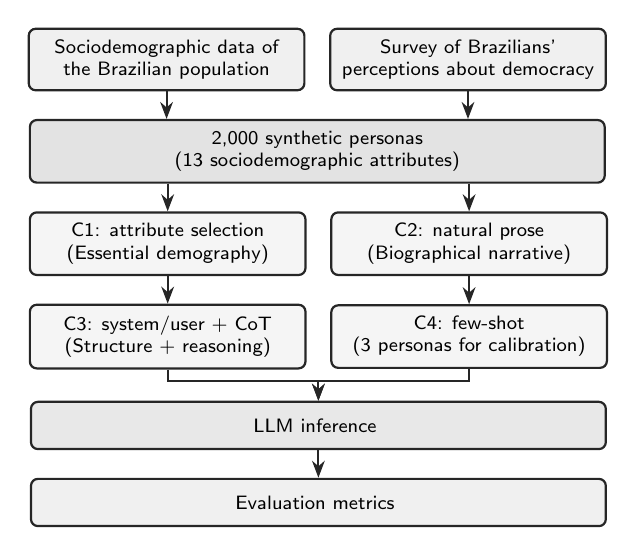
\begin{tikzpicture}[
    font=\sffamily\scriptsize,
    >=Stealth,
    baseBox/.style={
        rectangle,
        rounded corners=2.5pt,
        draw=black!85,
        line width=0.8pt,
        align=center,
        inner sep=4pt
    },
    dados/.style={baseBox, fill=gray!12, minimum width=3.5cm, minimum height=0.6cm},
    personas/.style={baseBox, fill=gray!22, minimum width=7.3cm, minimum height=0.6cm},
    scenario/.style={baseBox, fill=gray!8, minimum width=3.5cm, minimum height=0.6cm},
    llm/.style={baseBox, fill=gray!18, minimum width=7.3cm, minimum height=0.6cm},
    metrics/.style={baseBox, fill=gray!12, minimum width=7.3cm, minimum height=0.6cm},
    seta/.style={->, line width=0.7pt, draw=black!85}
]

    % --- 1. Data sources ---
    \node[dados] (ibge) {Sociodemographic data of\\the Brazilian population};
    \node[dados, right=0.3cm of ibge] (cesop) {Survey of Brazilians'\\perceptions about democracy};

    % --- 2. Synthetic personas ---
    \node[personas, below=0.35cm of $(ibge.south)!0.5!(cesop.south)$, align=center] (personas) {
        2,000 synthetic personas\\(13 sociodemographic attributes)
    };

    % --- 3. Prompt scenarios ---
    \node[scenario, below=0.35cm of personas.south west, anchor=north west, align=center] (c1) {
        C1: attribute selection\\(Essential demography)
    };
    \node[scenario, right=0.3cm of c1, align=center] (c2) {
        C2: natural prose\\(Biographical narrative)
    };
    \node[scenario, below=0.35cm of c1, align=center] (c3) {
        C3: system/user + CoT\\(Structure + reasoning)
    };
    \node[scenario, right=0.3cm of c3, align=center] (c4) {
        C4: few-shot\\(3 personas for calibration)
    };

    % --- 4. Inference and metrics ---
    \node[llm, below=0.4cm of $(c3.south)!0.5!(c4.south)$, align=center] (llms) {
        LLM inference
    };
    \node[metrics, below=0.35cm of llms.south, align=center] (metrics) {
        Evaluation metrics
    };

    % --- Connections ---
    \draw[seta] (ibge.south) -- (personas.north -| ibge.south);
    \draw[seta] (cesop.south) -- (personas.north -| cesop.south);

    \draw[seta] (personas.south -| c1.north) -- (c1.north);
    \draw[seta] (personas.south -| c2.north) -- (c2.north);

    \draw[seta] (c1.south) -- (c3.north);
    \draw[seta] (c2.south) -- (c4.north);

    \draw[seta] (c3.south) |- ++(0, -0.15) -| (llms.north);
    \draw[seta] (c4.south) |- ++(0, -0.15) -| (llms.north);

    \draw[seta] (llms.south) -- (metrics.north);
\end{tikzpicture}

    \caption{Methodological pipeline diagram, illustrating the experimental
        progression across prompt engineering stages.}
    \label{fig:pipeline}
\end{figure}

We structured the experimental investigation into two sequential and
complementary phases. Phase~1 evaluated the cumulative impact of four
prompt engineering strategies on distributional convergence, using a single
high-cardinality anchor question (P02) to isolate prompting effects.
Building upon the optimal prompt configuration identified in the first stage,
Phase~2 conducted an architectural benchmark comparing Brazilian
Portuguese-centric models against general-purpose global baselines across three
distinct thematic dimensions (P02, P03, and P04) to assess sociocultural fidelity
and generalization. The subsequent subsections detail the empirical reference
data, the synthetic population generation, the evaluated architectures, and
the experimental prompt scenarios.

\subsection{Empirical Reference Survey: Perceptions of Democracy}
\label{subsec:database}

We adopted the public opinion survey ``Perceptions of Brazilians Regarding
Democracy''~\cite{cesop04832} as our empirical ground truth. Fielded in September
2023 by the Center for Public Opinion Research (CESOP/UNICAMP) in partnership
with IPEC, the survey sampled 2,000 voting-age citizens across 127 Brazilian
municipalities using a three-stage probabilistic cluster design with quota
allocation based on official census indicators (margin of error of $\pm 2\%$ at a
95\% confidence level).

From the survey questionnaire, we selected three evaluative attitudinal
questions for comparative evaluation: P02 (Policy Priorities: ``Which of
these proposals do you think should be the priority of a politician?'',
featuring 12 substantive response alternatives); P03 (Fake News
Countermeasures: ``Which of these options do you believe could contribute to
combating the spread of fake news?'', with 6 substantive alternatives on regulatory and
institutional interventions); and P04 (Political Participation: ``Would you
say that you have a strong desire, some desire, or no desire to participate in
the political life of your city?'', offering 3 substantive alternatives measuring local civic
engagement).

Our selection includes all evaluative attitudinal items from the instrument,
deliberately omitting item P01 due to its purely retrospective nature as an
electoral recall check on 2022 voting behavior. This tripartite set provides
thematic breadth, spanning material policy agendas, institutional responses
to misinformation, and subjective civic disposition, while also varying in
response structure. By varying response cardinality across $12$, $6$, and
$3$ substantive categories, these questions allow us to evaluate JSD convergence under
different levels of response entropy and potential social desirability effects.

\subsection{Generation of the Synthetic Population Grounded in IBGE}
\label{subsec:silicon_profiles}

We generated 2,000 synthetic individual profiles using stratified
probabilistic sampling based on official distributions from the IBGE (Brazilian
Institute of Geography and Statistics), retrieved via the SIDRA
API~\cite{ibge_sidra_api}. Each persona is characterized by up to 13 attributes
spanning demographic, economic, and social dimensions, parameterized from the
2022 Demographic Census~\cite{ibge_censo_2022} (gender, age bracket, race,
region, zone, and religion), Continuous PNAD 2024~\cite{ibge_pnadc} (education,
employment, and \textit{per capita} income), the National Health Survey (PNS
2019)~\cite{ibge_pns_2019}, Civil Registry~\cite{ibge_registro_civil}, and
IPCA inflation indicators~\cite{ibge_ipca}.

Grounding the synthetic population directly in official IBGE microdata
guarantees reproducible probabilistic sampling across Brazilian federative units
and socioeconomic strata, ensuring the methodology remains transferable to
scenarios where prior survey ground truth does not pre-exist.

\subsection{Evaluated Large Language Model Architectures}
\label{subsec:language_models}

We compared four LLM architectures throughout our experiments, as summarized in
Table~\ref{tab:modelos}.

\begin{table}[htbp]
    \centering
    \caption{Large Language Models evaluated in the study.}
    \label{tab:modelos}
    \begin{tabular}{@{}llll@{}}
        \toprule
        \textbf{Model} & \textbf{Provider} & \textbf{Type} & \textbf{Origin} \\
        \midrule
        Sabiá-4 & Maritaca AI & API & Brazilian \\
        Sabiazinho-4 & Maritaca AI & API & Brazilian \\
        GPT-5-mini & OpenAI & API & Global \\
        LLaMA~3.2~3B & Meta & Local & Global \\
        \bottomrule
    \end{tabular}
\end{table}

The choice of Brazilian models (Sabiá-4 and Sabiazinho-4)
was grounded in the hypothesis that models pre-trained with an emphasis on the
Portuguese language and Brazilian sociocultural context could reproduce local
public opinion with higher fidelity. We selected GPT-5-mini as a
global baseline in the equivalent cost-performance tier, consistent with
the technical benchmark released by Maritaca AI for the Sabiá
architecture~\cite{abonizio_sabia-3_2024}.

\subsection{Experimental Prompt Engineering Strategies}
\label{subsec:cenarios}

We executed a cumulative progression of four experimental scenarios applying
incremental refinements to the prompt design strategy. In all scenarios, we
utilized 2,000 synthetic personas and initially focused on question
P02 (Policy Priorities). To mitigate the impact of probabilistic
sampling during inference, we repeated each prompt execution five times and
adopted the majority vote outcome for evaluation.

\subsubsection{Scenario 1: Feature Selection}
\label{subsubsec:cenario1}

In the first scenario, we applied a feature selection technique by using the
LLM itself to identify the most predictive variables among the
13 original attributes for the question at hand. For P02,
the model selected seven attributes: education,
\textit{per capita} income, region, age bracket,
self-rated health, gender, and marital status.

We structured the prompt as a single user message, presenting the profile as a
list within XML tags and requesting solely the letter corresponding to the
chosen alternative:

\begin{quote}
    \small
    \textit{``You must think and respond as a Brazilian citizen with the profile
    below. [\ldots] Consider the socioeconomic and demographic conditions of the
    profile to form your opinion on the question and respond with the letter of
    the alternative that best represents your opinion. [\ldots] My answer is''}
\end{quote}

We set the temperature to 0.7 and \texttt{max\_tokens} to
100, enforcing structured schema output (\texttt{response\_format}) to
ensure automated extraction.

\subsubsection{Scenario 2: Natural Prose Biographical Representation}
\label{subsubsec:cenario2}

As a natural evolution of the previous scenario, we utilized role-playing
techniques to assess how the model interpreted the presented profile. We
rephrased the prompt from a list of attributes into a natural language
descriptive paragraph:

\begin{quote}
    \small
    \textit{``Act as a Brazilian individual of gender [gender], from the [region]
    region, aged between [age bracket], [marital status]. Your education level is
    [education] and your individual income is [income]. Your self-rated health is
    [health].''}
\end{quote}

The remaining parameters (temperature, response format, and model) were kept
identical to Scenario~1.

\subsubsection{Scenario 3: Structural Role Separation and Chain of Thought (CoT)}
\label{subsubsec:cenario3}

In this scenario, we introduced two complementary structural modifications.
First, for \textit{role separation}, we allocated the persona profile and
behavioral guidelines exclusively to the \textit{system prompt}, providing the
question and alternatives in the \textit{user prompt}, reinforced by explicit
instructions to prevent breaking character: \textit{``Your task is to answer
public opinion questions exactly as this person would answer --- not as you
believe is correct, nor as an expert would answer.''} Second, to implement
\textit{Chain of Thought (CoT)}, we instructed the model to reflect briefly on how
an individual with the described profile would experience the issues in daily life
before selecting the final alternative, enforcing a structured response schema
with two fields: \texttt{reasoning} and \texttt{answer}.

We set the temperature to $0.9$ and adjusted \texttt{max\_tokens} to 200 to
allow for intermediate reasoning generation. Additionally, we reintroduced all
13 original profile attributes into the \textit{system prompt}.

\subsubsection{Scenario 4: Contextual Few-Shot Calibration}
\label{subsubsec:cenario4}

In the final scenario, we maintained the system/user prompt structure from
Scenario~3 and added three contrasting calibration personas as prior conversational
turns (assistant/user) preceding the target question. Specifically, the calibration
exemplars comprised: (1)~a young, low-income Black woman from the urban Northeast
choosing \textit{``Combat prejudice''} (alternative~b); (2)~an older, rural White
Evangelical man from the South choosing \textit{``Preserve family-oriented values''}
(alternative~g); and (3)~a middle-aged, college-educated divorced woman from the
urban Southeast choosing \textit{``Reduce social inequalities''} (alternative~a).

We constructed these three examples from qualitative analysis of
justifications generated by the LLM in previous runs (Scenario~3),
reusing them across all 2,000 simulations. We configured the structured
output to require three fields: \texttt{top\_concern} (primary daily concern),
\texttt{why\_this\_answer} (perspective justification), and \texttt{answer}
(alternative letter).

We appended an instruction to the end of the system prompt to mitigate inherent
training bias:

\begin{quote}
    \small
    \textit{``ATTENTION: In the real Brazil, surveys show that different
    Brazilians choose very different priorities. Prejudice, Inequality, Family
    values, Education, and Political participation are equally legitimate and
    frequent priorities. Health and Jobs are important to everyone, but they are
    not automatically the answer for every persona.''}
\end{quote}

To evaluate distributional convergence between simulated distributions ($P$)
and empirical CESOP targets ($Q$), response category counts were normalized to
unit sum ($\sum p_i = \sum q_i = 1$) and evaluated using base-2 Jensen-Shannon
Divergence (JSD)~\cite{lin_divergence_1991}. Bounded within $[0, 1]$ bit,
$\text{JSD} = 0$ denotes identical distributions. In line with computational
social simulation standards~\cite{miranda_simulating_2025}, we adopt $\text{JSD}
< 0.15$ as the threshold indicating close distributional convergence, whereas
values exceeding $0.50$ indicate severe empirical divergence.



\section{Results and Discussion}\label{sec:results}
\subsection{Distributional Evolution via Prompt Engineering}
\label{subsec:resultados_prompts}

Table~\ref{tab:resultados_prompts} presents the evolution of the
Jensen-Shannon Divergence (JSD) across the four experimental scenarios for
question P02 (Policy Priorities), utilizing the Sabiazinho-4 model.

\begin{table}[htbp]
    \centering
    \caption{JSD evolution across experimental scenarios (P02~--- Policy
        Priorities, Sabiazinho-4 model).}
    \label{tab:resultados_prompts}
    \begin{tabular}{@{}llcc@{}}
        \toprule
        \textbf{Scenario} & \textbf{Applied Technique} & \textbf{JSD} & \textbf{$\Delta$JSD} \\
        \midrule
        \textit{Baseline} & Raw \textit{prompt} (13 attributes) & 0.525 & --- \\
        Scenario 1 & Feature selection (7 attr.) & 0.366 & $-0.159$ \\
        Scenario 2 & Natural prose \textit{prompt} & 0.366 & $0.000$ \\
        Scenario 3 & \textit{System/User} + CoT & 0.297 & $-0.069$ \\
        Scenario 4 & \textit{Few-shot} (3 personas) & 0.121 & $\mathbf{-0.176}$ \\
        \bottomrule
    \end{tabular}
\end{table}

We observed an overall reduction of 77\% in JSD between the
\textit{baseline} ($0.525$) and the best experimental scenario ($0.121$), as
illustrated in Figure~\ref{fig:evolucao_jsd}. Feature selection (Scenario~1)
produced an immediate and substantial improvement ($\Delta\text{JSD} = -0.159$),
indicating that eliminating informational noise helps the model anchor its
decisions on the most decisive variables. Natural prose reformatting
(Scenario~2) maintained the identical JSD value, suggesting that textual syntax
alone does not alter the output probability distribution. Conversely, the Chain
of Thought reasoning (Scenario~3) promoted a significant incremental gain
($\Delta\text{JSD} = -0.069$). Finally, introducing calibration examples
(\textit{few-shot}, Scenario~4) allowed the simulation to surpass the target
threshold of distributional convergence ($\text{JSD} < 0.15$), reaching
$0.121$.

\begin{figure}[htbp]
    \centering
    \resizebox{\columnwidth}{!}{%
        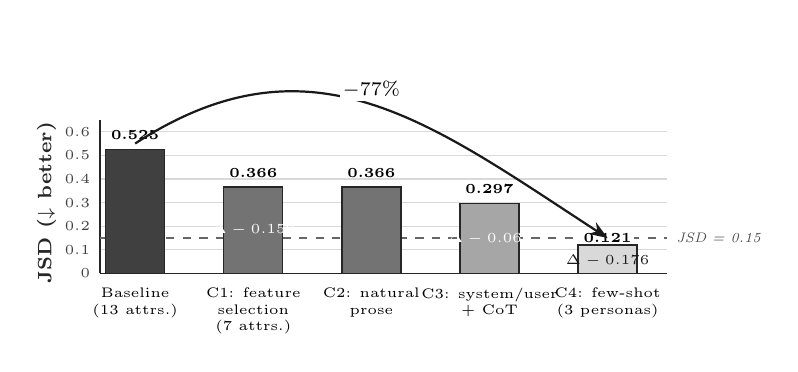
\begin{tikzpicture}[
    font=\sffamily\scriptsize,
    xscale=1.5,
    yscale=3.0,
    bar/.style={draw=black!85, line width=0.5pt},
    refline/.style={dashed, draw=black!60, line width=0.5pt},
    label/.style={font=\tiny\bfseries}
]

    % --- Y-axis grid ---
    \foreach \y in {0.0, 0.1, 0.2, 0.3, 0.4, 0.5, 0.6} {
        \draw[black!15, line width=0.4pt] (-0.3, \y) -- (4.5, \y);
        \node[left, font=\tiny, text=black!75] at (-0.3, \y) {\pgfmathprintnumber[fixed,precision=1]{\y}};
    }
    \draw[black!85, line width=0.6pt] (-0.3,0) -- (4.5,0);
    \draw[black!85, line width=0.6pt] (-0.3,0) -- (-0.3,0.65);
    \node[rotate=90, font=\scriptsize\bfseries, text=black!85] at (-0.75, 0.30) {JSD ($\downarrow$ better)};

    % --- Reference line ---
    \draw[refline] (-0.3, 0.15) -- (4.5, 0.15);
    \node[right, font=\tiny\itshape, text=black!70] at (4.5, 0.15) {JSD = 0.15};

    % --- Scenario bars ---
    \filldraw[bar, fill=black!75] (-0.25, 0) rectangle (0.25, 0.525);
    \node[above, label] at (0, 0.525) {0.525};
    \node[below, font=\tiny, align=center] at (0, -0.02) {Baseline\\(13 attrs.)};

    \filldraw[bar, fill=black!55] (0.75, 0) rectangle (1.25, 0.366);
    \node[above, label] at (1.0, 0.366) {0.366};
    \node[font=\tiny\bfseries, text=white] at (1.0, 0.183) {$\Delta -0.159$};
    \node[below, font=\tiny, align=center] at (1.0, -0.02) {C1: feature\\selection\\(7 attrs.)};

    \filldraw[bar, fill=black!55] (1.75, 0) rectangle (2.25, 0.366);
    \node[above, label] at (2.0, 0.366) {0.366};
    \node[below, font=\tiny, align=center] at (2.0, -0.02) {C2: natural\\prose};

    \filldraw[bar, fill=black!35] (2.75, 0) rectangle (3.25, 0.297);
    \node[above, label] at (3.0, 0.297) {0.297};
    \node[font=\tiny\bfseries, text=white] at (3.0, 0.148) {$\Delta -0.069$};
    \node[below, font=\tiny, align=center] at (3.0, -0.02) {C3: system/user\\+ CoT};

    \filldraw[bar, fill=black!15] (3.75, 0) rectangle (4.25, 0.121);
    \node[above, label, fill=white, inner sep=0.8pt] at (4.0, 0.121) {0.121};
    \node[font=\tiny\bfseries, text=black!90] at (4.0, 0.055) {$\Delta -0.176$};
    \node[below, font=\tiny, align=center] at (4.0, -0.02) {C4: few-shot\\(3 personas)};

    % --- Global reduction ---
    \draw[->, >=Stealth, line width=0.8pt, draw=black!90] (0.0, 0.55) to[out=18, in=162] node[above=1pt, font=\scriptsize\bfseries, fill=white, inner sep=1pt] {$-77\%$} (4.0, 0.15);
\end{tikzpicture}
%
    }
    \caption{JSD evolution across prompt engineering scenarios (P02,
        Sabiazinho-4), demonstrating a 77\% reduction from baseline to
        Scenario~4 (few-shot).}
    \label{fig:evolucao_jsd}
\end{figure}

\subsection{Systematic Benchmark: Brazilian Portuguese-Centric vs. Global Models}
\label{subsec:resultados_modelos}

Table~\ref{tab:resultados_modelos} summarizes the comparative performance of
the four evaluated models (Sabiá-4, Sabiazinho-4, GPT-5-mini, and
LLaMA~3.2~3B) across the three target questions (P02, P03, and P04).

\begin{table}[htbp]
    \centering
    \begin{threeparttable}
        \caption{Comparative performance of models across questions using JSD.}
        \label{tab:resultados_modelos}
        \setlength{\tabcolsep}{6pt}
        \begin{tabular}{@{}llc@{}}
            \toprule
            \textbf{Question} & \textbf{Model} & \textbf{JSD ($\downarrow$)} \\
            \midrule
            \multirow{4}{*}{\shortstack[l]{P02: Policy\\Priorities}}
                & Sabiá-4 & 0.7238 \\
                & Sabiazinho-4 & 0.5664 \\
                & GPT-5-mini & 0.6185 \\
                & LLaMA~3.2~3B & \textbf{0.4882} \\
            \midrule
            \multirow{4}{*}{\shortstack[l]{P03: Fake\\News}}
                & Sabiá-4 & 0.6846 \\
                & Sabiazinho-4 & \textbf{0.5452} \\
                & GPT-5-mini & 0.5908 \\
                & LLaMA~3.2~3B & 0.5912 \\
            \midrule
            \multirow{4}{*}{\shortstack[l]{P04: Political\\Participation}}
                & Sabiá-4 & 0.3007 \\
                & Sabiazinho-4 & \textbf{0.2097} \\
                & GPT-5-mini & 0.8263 \\
                & LLaMA~3.2~3B & 0.8100 \\
            \midrule
            \multirow{4}{*}{\shortstack[l]{Mean JSD\\($\overline{\text{JSD}}$)}}
                & Sabiazinho-4 & \textbf{0.4404} \\
                & Sabiá-4 & 0.5697 \\
                & LLaMA~3.2~3B & 0.6298 \\
                & GPT-5-mini & 0.6785 \\
            \midrule
            \multicolumn{2}{@{}l}{\textbf{Overall Mean $\pm$ SD}} & \textbf{0.5796 $\pm$ 0.1839} \\
            \bottomrule
        \end{tabular}
        \begin{tablenotes}
            \footnotesize
            \item \textit{Note:} $\downarrow$ indicates that lower values denote
                closer alignment to the real CESOP distribution (JSD). Bold indicates best performance per question and overall mean.
        \end{tablenotes}
    \end{threeparttable}
\end{table}

The aggregated comparative analysis reveals that Sabiazinho-4 achieved
the best average distributional adherence ($\overline{\text{JSD}} = 0.4404$),
followed by Sabiá-4 ($\overline{\text{JSD}} = 0.5697$),
LLaMA~3.2~3B ($\overline{\text{JSD}} = 0.6298$), and
GPT-5-mini ($\overline{\text{JSD}} = 0.6785$).

Analyzing results across individual questions (Table~\ref{tab:resultados_modelos}) demonstrates
that simulation accuracy is strongly conditioned by thematic domain characteristics.
On the one hand, Question P04 (Political Participation) revealed the most pronounced
polarization between model families: Brazilian architectures exhibited high empirical
alignment ($\text{JSD} = 0.2097$ for Sabiazinho-4 and $0.3007$ for Sabiá-4), whereas
global baselines failed substantially ($\text{JSD} = 0.8263$ for GPT-5-mini and
$0.8100$ for LLaMA~3.2~3B) due to acute social desirability bias. On the other hand,
Questions P02 and P03 (Policy Priorities and Fake News) showed moderate dispersion
across all models ($\text{JSD}$ between $0.48$ and $0.72$), reflecting their larger
combinatorial choice spaces (14 and 8 alternatives) and underlying socioeconomic
complexity.

Regarding cross-consistency across questions and models, Sabiazinho-4
maintained superior stability across all thematic dimensions, avoiding the
severe degradation peaks observed in globally aligned models
(Table~\ref{tab:resultados_modelos}).

\subsection{Sociocultural Biases, Explainability Auditing, and Methodological Trade-offs}
\label{subsec:discussao_qualitativa}

Detailed inspection of simulated distributions revealed systematic bias
patterns conditioned by model origin and training alignment. Brazilian
architectures (Sabiá-4 and Sabiazinho-4) demonstrated appropriate sensitivity to
the civic skepticism of the Brazilian electorate in P04, accurately capturing
the substantial proportion of respondents expressing little or no desire to
participate in municipal politics. However, in P02, they exhibited a tendency to
over-prioritize healthcare quality, occasionally assigning it to higher-income
personas holding private health insurance. Conversely, global models (GPT-5-mini
and LLaMA~3.2~3B) displayed pronounced social desirability and institutional
optimism biases: in P04, GPT-5-mini attributed positive participation desire to
over 98\% of synthetic personas, failing to reproduce documented political
alienation, while responses in P02 heavily concentrated on job creation in a
standard corporate/institutional style.

Incorporating intermediate reasoning (Chain-of-Thought) in Scenario~3 enabled
qualitative auditing of persona decision processes, resolving the opacity
inherent in unreasoned prompts. Qualitative inspection of explanatory rationales
unveiled two primary phenomena. First, genuine demographic alignment occurred
when models anchored decisions at the intersection of income, education, and
geography (for instance, lower-income, less-educated personas articulating civic
disengagement due to perceived institutional corruption and distance). Second,
persona dissonance emerged when models conflated simulated profiles with generic
knowledge (such as affluent personas holding private coverage selecting public
healthcare improvements due to broader societal perceptions of health system
precarity). This transparency establishes XAI not merely as a \textit{post hoc}
validation tool, but as an active diagnostic instrument for auditing behavioral
coherence in synthetic populations.

Finally, while Scenario~4 attained optimal distributional convergence ($\text{JSD} =
0.121$), introducing manual calibration examples entails an essential
methodological trade-off: in-context demonstrations serve as potent
distributional anchors, requiring balanced selection to prevent steering models
toward researcher priors.


\section{Conclusions and Future Work}\label{sec:conclusion}
In this paper, we demonstrate that structured prompt engineering exerts a
decisive impact on the capability of Large Language Models to simulate empirical
public opinion distributions in Brazil. Our findings establish that cumulative
prompt refinement progressively minimizes distributional divergence, achieving
optimal alignment ($\text{JSD} = 0.121$) through the synergy of demographic
feature selection, structural role separation, Chain-of-Thought deliberation,
and in-context calibration. Furthermore, our innovative benchmarking between
culturally specialized Brazilian architectures (Sabiá-4 and Sabiazinho-4) and
general-purpose global baselines (GPT-5-mini and LLaMA~3.2~3B) reveals that
domain-tailored models exhibit superior sociocultural fidelity by accurately
capturing empirical civic skepticism, whereas global baselines succumb to severe
social desirability and institutional optimism biases. Within this framework,
Explainable AI (XAI) auditing proves indispensable for detecting cognitive
dissonance and verifying persona behavioral consistency.

The authors acknowledge, however, certain methodological limitations of these
findings. Most notably, the empirical benchmark relies on a single
cross-sectional survey instrument (CESOP/IPEC) centered on democratic
perceptions. While this instrument provides rich structural variance across
multi-alternative policy, institutional, and engagement items, fully
consolidating the external validity of silicon sampling warrants replicating
this evaluative pipeline across broader thematic domains and longitudinal
polling cycles.

Promising avenues for future research involve deploying Retrieval-Augmented
Generation (RAG) to dynamically inject real-time regional context and exploring
supervised fine-tuning of open-weight architectures on authentic citizen
rationales. Extending this probabilistic framework across additional open-weight
foundations and sampling temperatures will further strengthen simulation
robustness. Ultimately, this work demonstrates the strong potential of Large
Language Models for public opinion simulation and establishes solid
methodological directions for their continued development.



\bibliographystyle{IEEEtran}
\bibliography{IEEEabrv,references}

\end{document}
